\chapter{Desarrollo.}
\section{Algoritmo de Buchberger.}
Para un mejor entendimiento del Algoritmo de Buchberger pensé que lo mejor sería programarlo para asi ver paso a paso su funcionamiento, con esta meta y una vez programado hice una versión que me diera una salida por pantalla que me permitiese hacer un seguimiento en cada iteración del Algoritmo. A continuación incluyo las dos versiones que he realizado así como la salida por pantalla de un ejemplo para ver funcionar el algoritmo.

\subsection{Versión para importar y usar.} 
\lstinputlisting[language=Python]{codigos/buchberger_no_exp.py}

\subsection{Versión explicada.} 
\lstinputlisting[language=Python]{codigos/buchberger_exp.py}

\section{Brazo.}
Para ver el uso de lo desarrollado a lo largo de esta memoria he realizado un pequeño programa en matplotlib el cual dibujará un brazo de dos articulaciones en un entorno 3D. Se podrá elegir mediante widgets tanto la posición final del brazo como si queremos que el brazo se mueva en el plano o en el espacio, es decir, si la articulación de la base es planar o universal.
He elegido usar matplotlib por la comodidad que me proporciona el uso de widgets y la buena representación 3D que realiza. Ahora pasaré a explicar el código y los detalles sobre él:

En principio importamos los paquetes necesarios y comenzamos a definir la única clase que vamos a tener, Draw\_Robot, dentro de la cual llevaremos todo acabo.
Empezamos con el constructor y vemos la definición de variables, a las longitudes (l) les he dado valor 100 y en principio la posición inicial(tx,ty,tz) será (0,100,100).
\lstinputlisting[language=Python,firstline=0,lastline=22]{codigos/brazo.py}
Seguimos dentro del constructor y ahora lo que vamos a hacer es preparar todo lo concerniente al calculo de nuestra base de Gröbner. Preparamos nuestras ecuaciones particulares para este caso:
\begin{eqnarray}
\nonumber &a-l3*(c1*c2-s1*s2)-l2*c1 \\
\nonumber &b-l3*(c1*s2+c2*s1)-l2*s1 \\
\nonumber &c1^2+s1^2-1 \\
\nonumber &c2^2+s2^2-1
\end{eqnarray}
Usamos groebner para estas ecuaciones, indicando que el orden va a ser lex y que el sistema resultante va a depender de s1,c1,s2,c2. 
\lstinputlisting[language=Python,firstline=23,lastline=27]{codigos/brazo.py}
Este sería el resultado:

\begin{lstlisting}
	GroebnerBasis([
	c2 + (-a**2 - b**2 + l2**2 + l3**2)/(2*l2*l3), 
	s2 + s1*(a**2 + b**2)/(a*l3) + (-a**2*b - b**3 - b*l2**2 + b*l3**2)/(2*a*l2*l3), 
	c1 + b*s1/a + (-a**2 - b**2 - l2**2 + l3**2)/(2*a*l2), 
	s1**2 + s1*(-a**2*b - b**3 - b*l2**2 + b*l3**2)/(a**2*l2 + b**2*l2) + (a**4 + 2*a**2*b**2 - 2*a**2*l2**2 - 2*a**2*l3**2 + b**4 + 2*b**2*l2**2 - 2*b**2*l3**2 + l2**4 - 2*l2**2*l3**2 + l3**4)/(4*a**2*l2**2 + 4*b**2*l2**2)], 
		c2, s2, c1, s1, domain='QQ(a,b,l2,l3)', order='lex')
\end{lstlisting}

Como vemos hay 4 ecuaciones que, teniendo en cuenta que a,b,l2 y l3 son conocidos, forman un sistema de ecuaciones triangular en el que la primera solo depende de c2, la cuarta de c2 y s1, la segunda de c2, s1 y s2 y la tercera de c2, s1, s2 y c1.

A continuación vamos resolviendo el sistema y obteniendo c2, s1, s2 y c1; quedando estas en funcion de a, b, l2 y l3. Una vez tengamos esto, será solamente necesaria una simple sustitución para tener los datos que necesitamos para dibujar el brazo.

\lstinputlisting[language=Python,firstline=28,lastline=37]{codigos/brazo.py}

Pasamos a ver el diseño de la ventana principal del programa, que nos ayudara a comprender el código mejor:

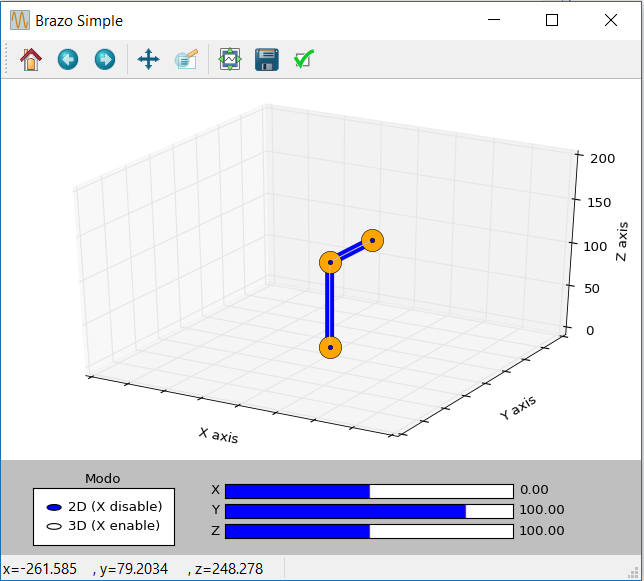
\includegraphics[scale=0.85]{imagenes/disenio_ventana}

Empezaremos creando la ventana(fig) con un nombre, y dentro de ella la ventana de dibujado(ax) y el panel de error(axerror).

\lstinputlisting[language=Python,firstline=38,lastline=42]{codigos/brazo.py}

Ahora crearemos los widgets que vamos a usar que, como se ve en la imagen, son tres Sliders, uno por coordenada y un Radio Button para cambiar de Modo, dejaremos el Slider de la X desactivado ya que inicialmente el Modo será 2D y por tanto se moverá en el plano X=0.

\lstinputlisting[language=Python,firstline=43,lastline=60]{codigos/brazo.py}

Después añadimos los manejadores de eventos de los 4 widgets. Cuando el valor de alguno de los  Sliders se actualizará el valor de las variables de clase tx, ty o tz, según de cual se haya modificado el valor, y se llamará a la función draw\_robot, la cuál veremos más adelante.
En el caso del manejador del Radio Button del Modo, este activará o desactivará el Slider X y cambiará la variable de clase modo.

\lstinputlisting[language=Python,firstline=62,lastline=90]{codigos/brazo.py}

Ya solo nos queda llamar a display\_error, a drow\_robot y hacemos show para dibujarlo todo.

\lstinputlisting[language=Python,firstline=91,lastline=95]{codigos/brazo.py}

Y con esto habríamos terminado el constructor, Ahora escribimos algunas funciones de la clase, empezando por preparar una señal de error que nos indicara cuando se le a solicitado al brazo acceder a una posición fuera de su alcance.

\lstinputlisting[language=Python,firstline=97,lastline=104]{codigos/brazo.py}

La función siguiente es la encargada de, usando todo lo preparado en el constructor y los valores introducidos por los Sliders, obtener los valores de c1,s1,c2,s2 y una vez comprobado que son números reales, si son imaginarios activamos el display\_error, actualizar los valores de y[1] y z[1]. Para hacer esto usaremos, de los dos valores posibles de s1, el positivo para así evitar problemas al cambiar de cuadrante.
También situaremos y[2] y z[2] en la posición elegida en los Sliders.

Tanto x[1], como x[2] serán puestas a 0 ya que esta función es para el modo 2D.

\lstinputlisting[language=Python,firstline=105,lastline=132]{codigos/brazo.py}

Para el caso en 3D vamos a usar un cambio a coordenadas esféricas, esto es:
\[
\left \{
\begin{array}{lll}
x = r\cdot sin(\theta)\cdot cos(\varphi)\\
y = r\cdot sin(\theta)\cdot sin(\varphi)\\
z = r\cdot(\varphi)
\end{array}
\right .
\left .
,\;siendo\; \varphi
\right .
=
\left \{
\begin{array}{lll}
arctan\left(\frac{y}{x}\right) 			& x>0\; y\; y>0\\
2\pi + arctan\left(\frac{y}{x}\right)	& x>0\; y\; y<0\\
\frac{\pi}{2}\cdot sgn(y)						& x=0\\
\pi + arctan\left(\frac{y}{x}\right) 	& x<0\\
\end{array}
\right .
\]


\lstinputlisting[language=Python,firstline=133,lastline=172]{codigos/brazo.py}

A continuación vemos las funciones set\_positions y set\_ax.
La primera será la que dibuje el robot, y la segunda la que dibuje el sistema de coordenadas.

\lstinputlisting[language=Python,firstline=173,lastline=193]{codigos/brazo.py}

Por último tenemos la función draw\_robot la cual tendrá en cuenta el modo para calcular Gröbner en 2D o en 3D y, tras estos cálculos, ver si estamos ante un estado posible o no. Si el estado es posible no dibujaremos la señal de error y dibujaremos tanto los ejes como el brazo y en caso contrario, solo dibujaremos el error.
Por ultimo hacemos draw para dibujar todo. 

\lstinputlisting[language=Python,firstline=194,lastline=207]{codigos/brazo.py}

Y ya fuera de la clase, tenemos el main que lo único que hace es crear un objeto Draw\_robot. 

\lstinputlisting[language=Python,firstline=209,lastline=250]{codigos/brazo.py}
